\documentclass{article}
\usepackage{graphicx}
\usepackage{forest}
\usepackage{float}
%A4 page size = 210mm, 297mm / inset total = size-margin
\usepackage[a4paper, total={180mm, 267mm}]{geometry}
\usepackage{fontspec}
%\setmainfont{Times New Roman}

\title{
  BSS310 Project \\
  GROUP 101 \\
}
\author{Authors:\\Jan-Hendrik Brink,  u23694956
                \\Derich Ben Havenga, u23536812
                \\Mundell Brown, u22637062 
}

\begin{document}
  \huge{\bfseries{PART B}}
   \begin{figure}[H]
    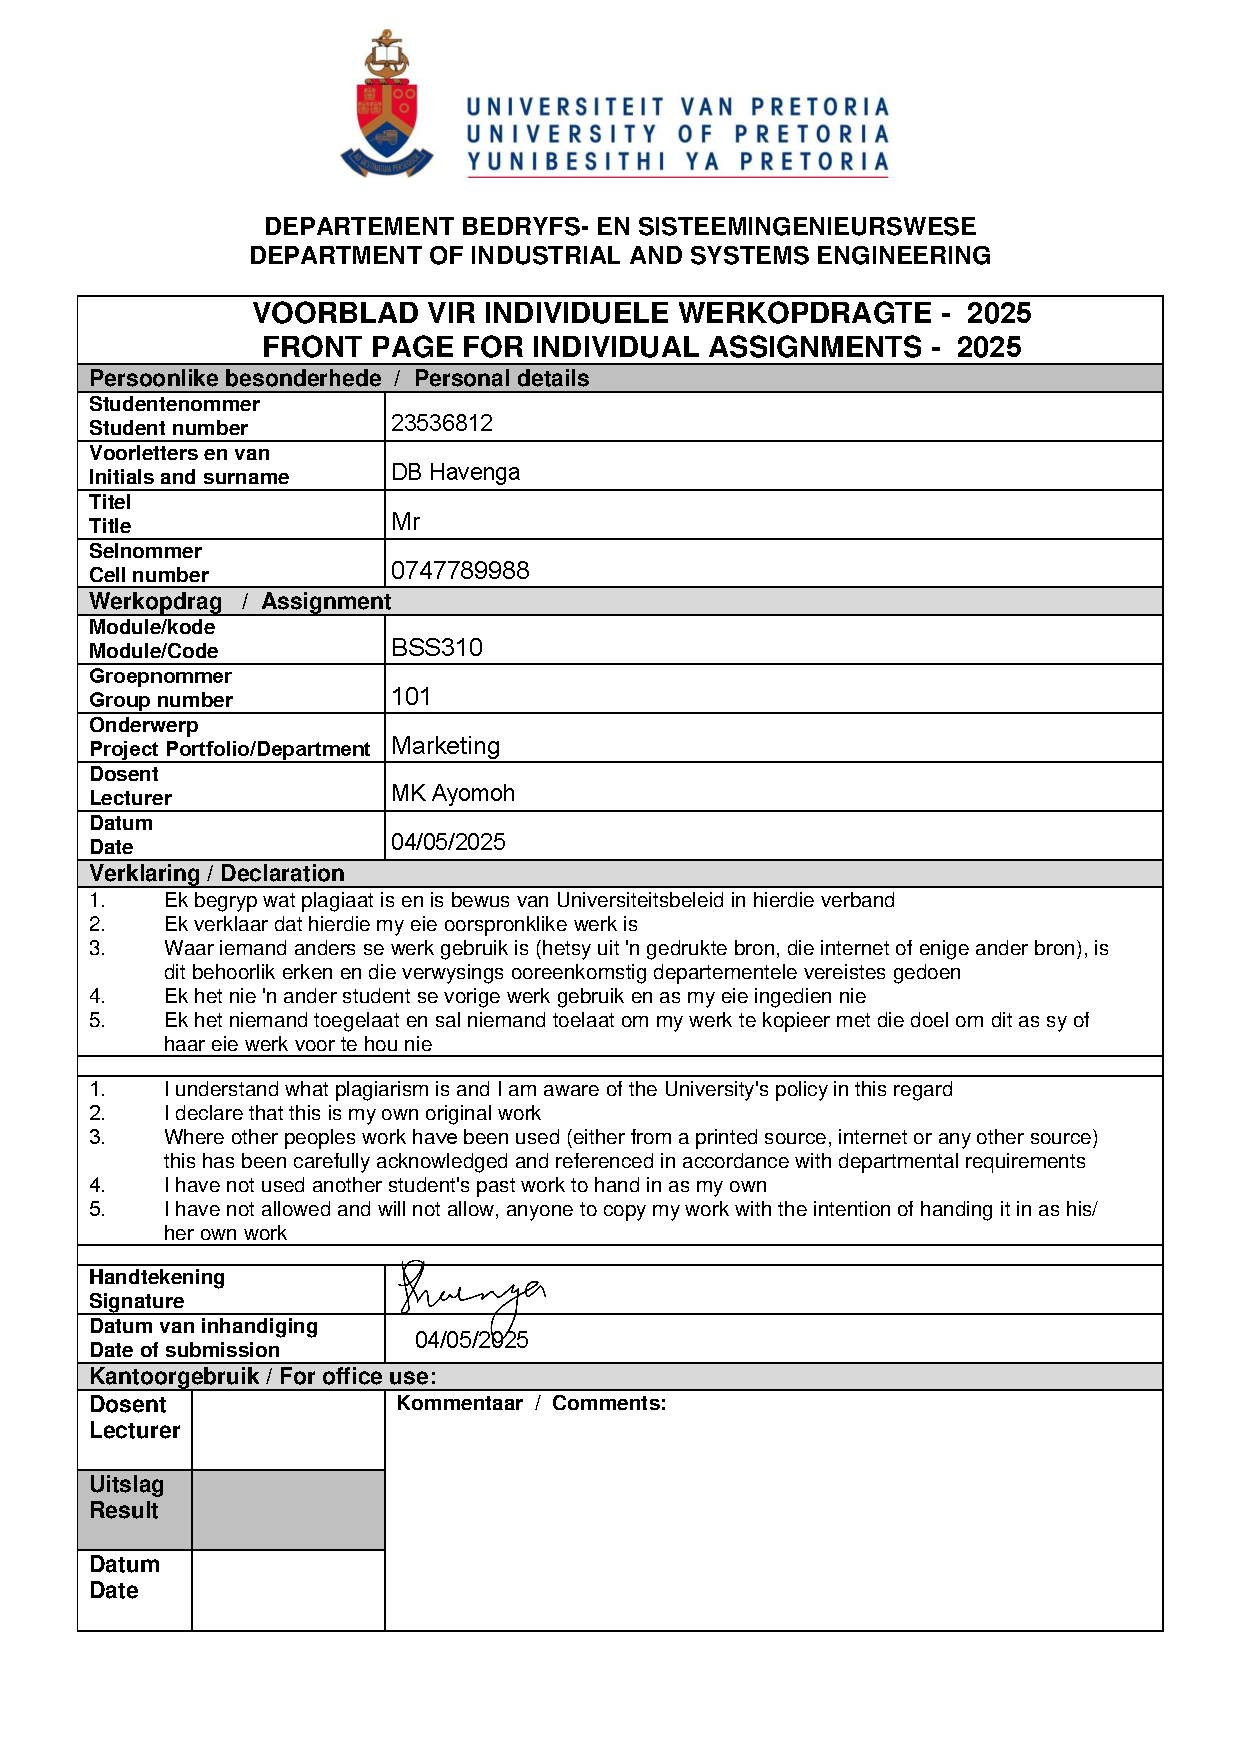
\includegraphics[width=1\linewidth]{figures/Cover_Page_Part_B_Derich.pdf}
  \end{figure}
  \newpage{} 
  \large Marketing portfolio by Derich Havenga (23536812)
  \large 
 \section{Description of System Characteristics based on its functional capabilities}
The marketing department's main goal is create a presence in the consumer market, and establish good relations with customers. The department will focus its efforts to market the product towards professionals who want to alleviate their ADHD symptoms. The system characteristics and the functions to achieve them are given in Table \ref{tab:system_char}

\begin{table}[H]
    \centering
    \caption{System characteristics of the Marketing department and their respective functions}
    \begin{tabular}{c|c}
         Characteristic & Functions  \\
         \hline
         Market planning & Identify target market, determine marketing objectives, create marketing tactics, plan project timeline \\
         Market research & Identify target markets needs and wants, identify marketing opportunities, identify marketing channels\\
         Market deployment & Create marketing campaign towards ADHD professionals, create social media following \\
         Orient customers & Create info-graphics, create guides to product, create an informational website \\
         Satisfy customers & Create and manage helpline, and FAQ page \\
        \hline
        \hline
    \end{tabular}
    \label{tab:system_char}
\end{table}
 \section{Project Scope and Stakeholders}
 The proper declaration of scope and identification of stakeholders are important for the planning and future operation of the marketing department.
 \subsection{Project Scope}
 The marketing department should complete proper research and planning before production and distribution set-up of the product is complete. Planning will include determining marketing objectives and formulating strategies to achieve the objectives. A timeline should be created where the goals and sub-goals are defined and scheduled. The research should include comprehensive analysis of the target market ( professionals diagnosed with ADHD), marketing opportunities and channels. 

The department will also be responsible for planning and deployment of advertisements and other marketing campaigns but not for production of marketing media as it will be outsourced to a marketing media company. An initial marketing campaign should be completed before distribution to retailers and stockists and monthly campaign should follow after. The department will deploy the campaigns via Google Ads and other online advertisement services. A social media page should also be created to target the younger workforce.

The marketing department is also tasked with creating a quality customer service. Customer service is vital and a high standard should be upheld during the length of the project. The customer services provided will include a customer care line, a FAQ page and an informational web page that will include a guide to properly use the product. 

 \subsection{Stakeholders}
The stakeholders for the marketing department, can be segmented into external and internal stakeholders. The internal stakeholders are: The founders, investors,  marketing team, production and logistics team. The external stakeholders are: Consumers, competitors, Top click media, Google Ads, HostAfrica, Takealot, and Dischem. Figure \ref{fig:stakeholder} shows a map of the stakeholders against level of interest and influence. 
 % stakeholder map
 \begin{figure}[H]
     \centering
     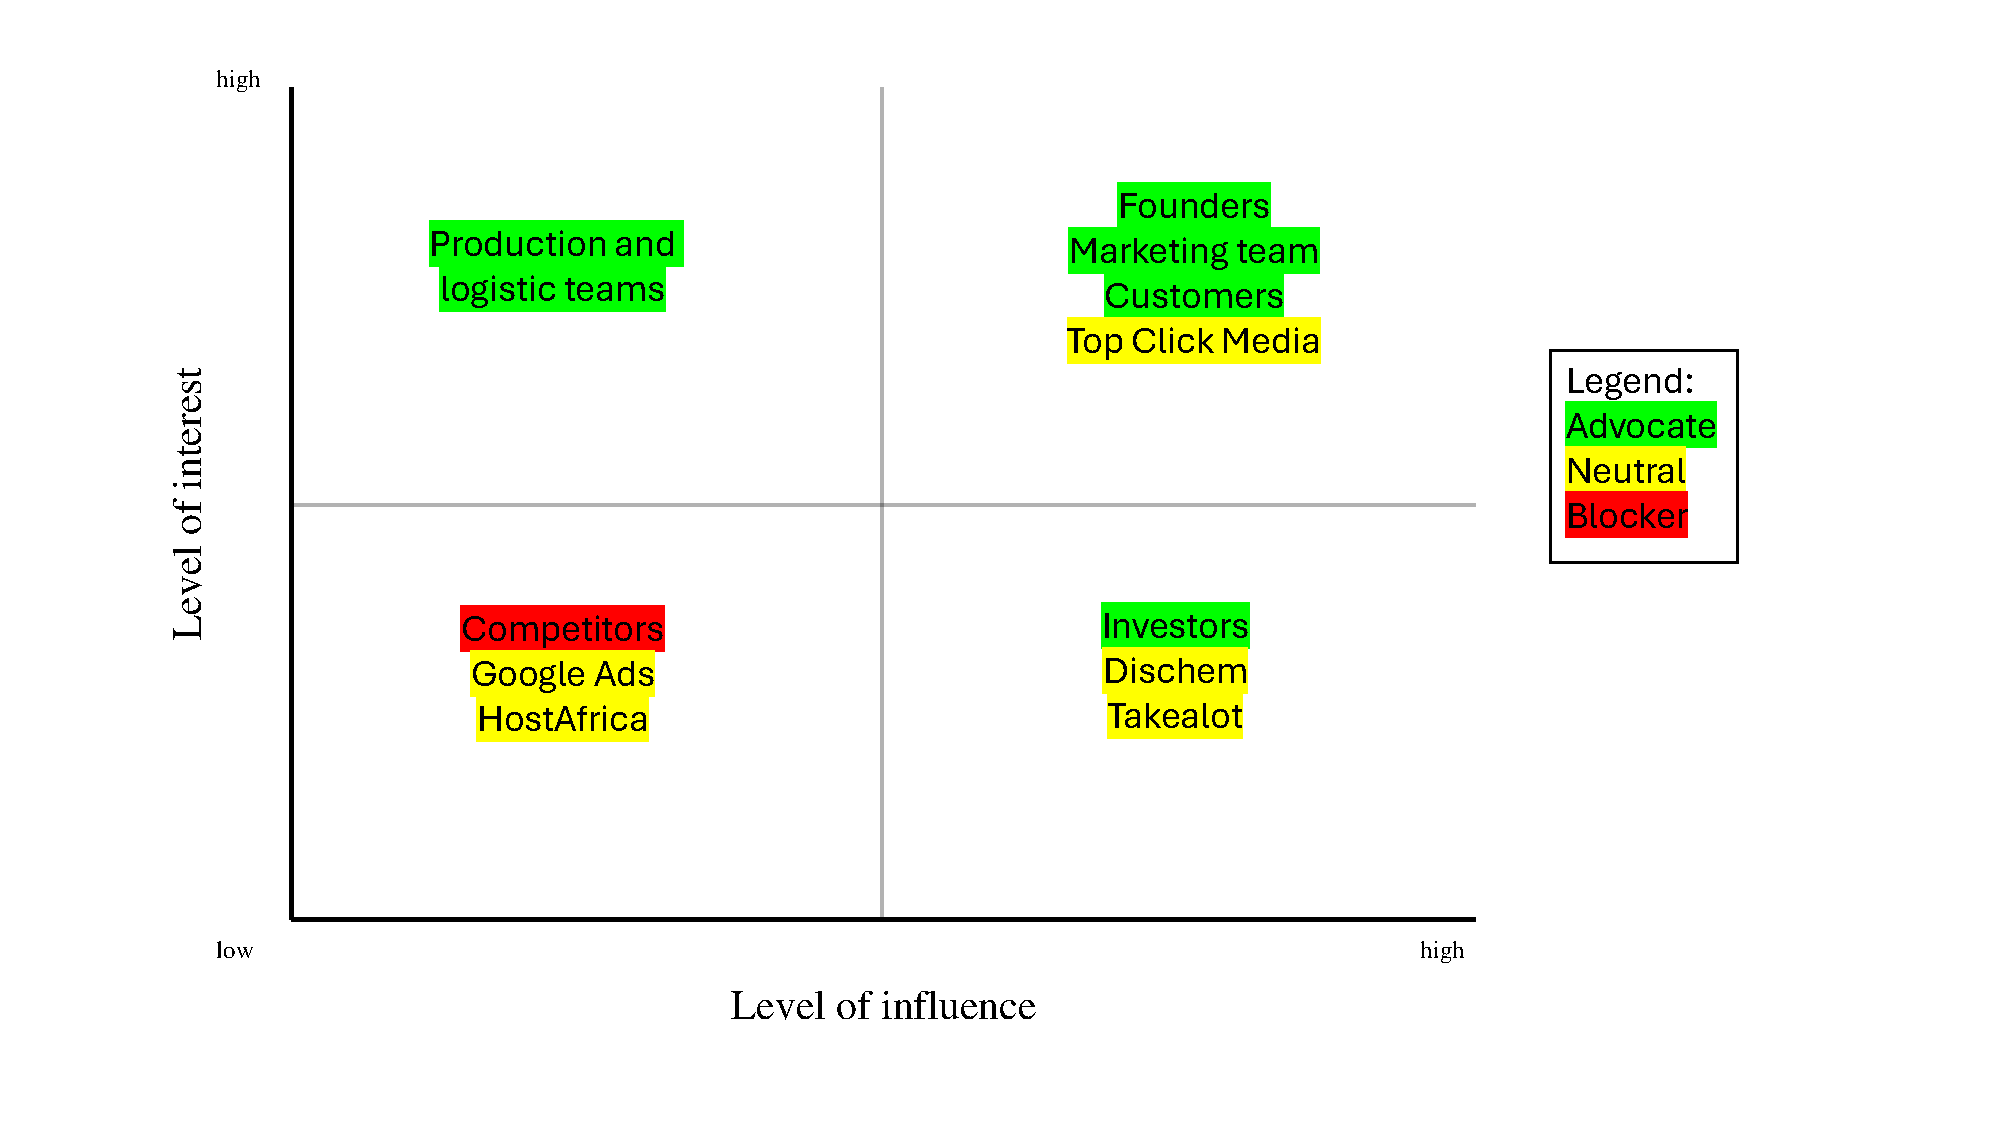
\includegraphics[width=0.75\linewidth]{figures/stakeholder map.pdf}
     \caption{Stakeholder map for the marketing department}
     \label{fig:stakeholder}
 \end{figure}
 
 \section{Project Plan}
 \subsection{Define the phases and deliverables of the project}
Table \ref{tab:phases} shows the phases and deliverables of the marketing project.
\begin{table}[H]
    \centering
    \caption{Project phases and deliverables for each respective phase}
    \begin{tabular}{c|c}
         Phase  & Deliverable  \\
         \hline
         Initialisation & Research report document, marketing plan and strategy document, marketing schedule, contracts\\
            Execution & Advertisements, social media pages, websites\\
        Re-evaluation & Future advertisement release schedule\\
         \hline
         \hline
    \end{tabular}
    
    \label{tab:phases}
\end{table}
 
 \subsection{Develop a work breakdown structure}
 Figure \ref{fig:WBS} shows the work breakdown structure for the department.
\begin{figure}[H]
    \centering
    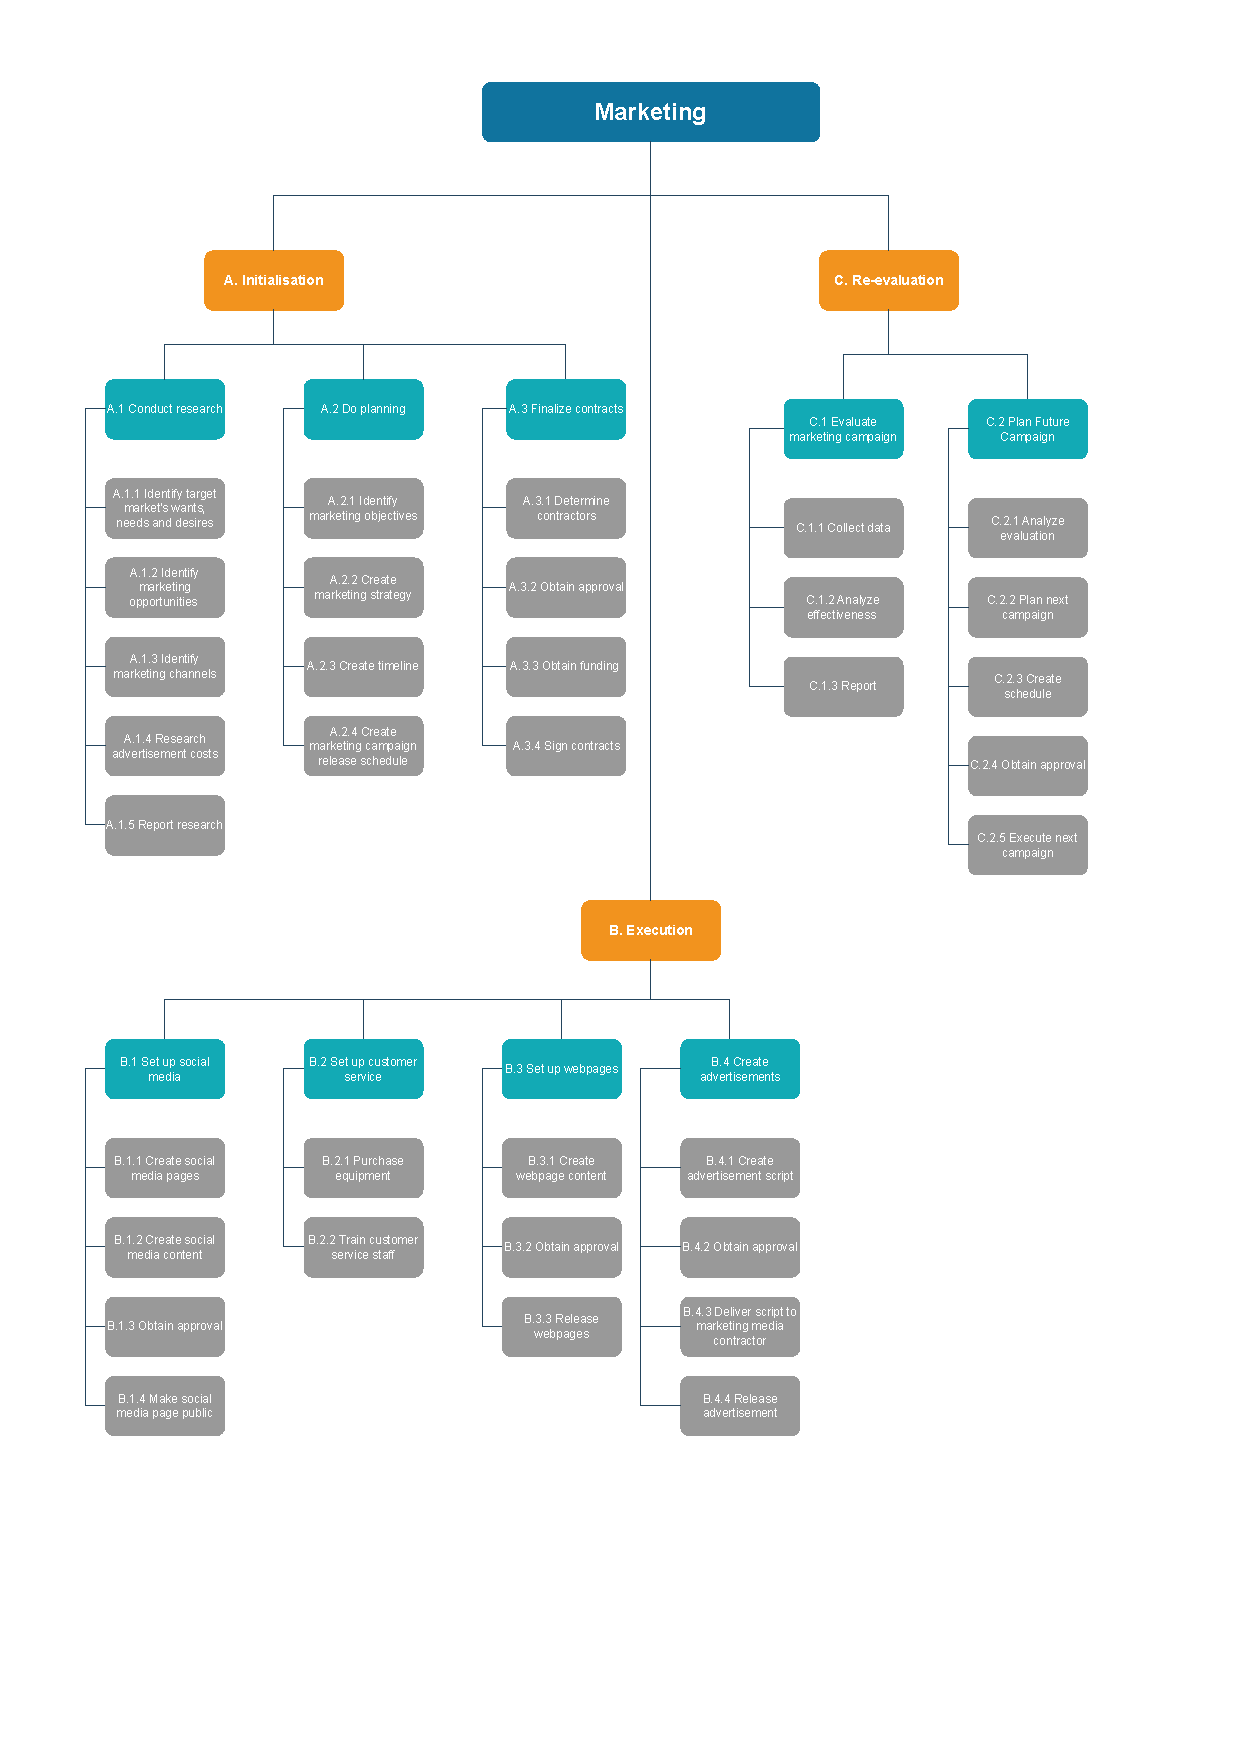
\includegraphics[width=0.75\linewidth]{figures/WBS.pdf}
    \caption{Work breakdown structure for the marketing department}
    \label{fig:WBS}
\end{figure}
 
 \subsection{Create a network diagram that indicates the critical path }
 Figure \ref{fig:network} shows the network diagram of the work breakdown structure, indicating earliest start, earliest finish, latest start, latest finish and the critical path.
\begin{figure} [H]
    \centering
    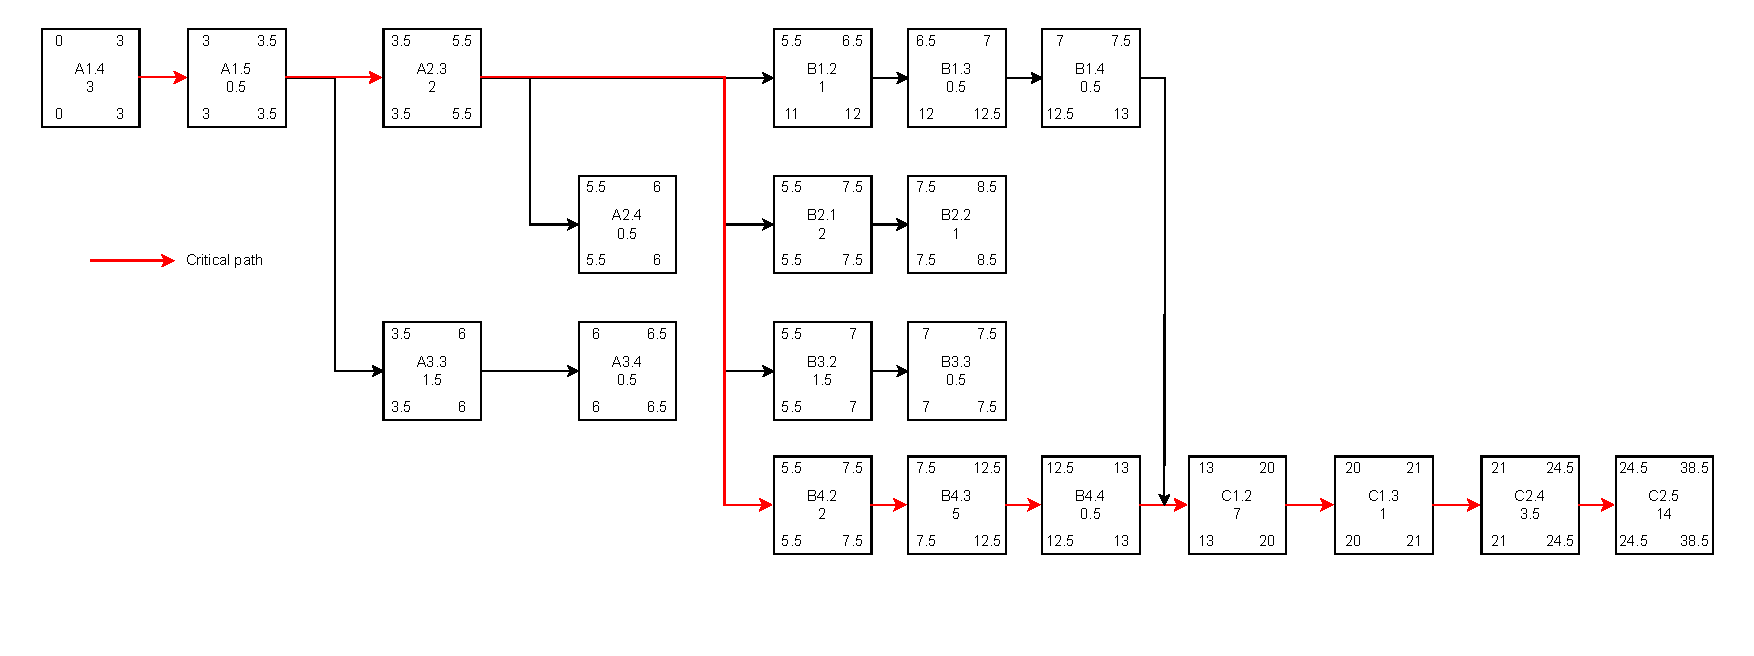
\includegraphics[width=0.75\linewidth]{figures/Network.pdf}
    \caption{Network diagram}
    \label{fig:network}
\end{figure}
 
 \subsection{Indicate the float, slack, forward pass and backward pass}
 Table \ref{tab:forward} indicates the forward and backward of Figure \ref{fig:network}. Table \ref{tab:Float} indicates the float and slack for each activity present in the network diagram.
\begin{table}[H]
    \centering
    \caption{Forward and backward pass}
    \begin{tabular}{c|cc}
                        & Start date & End date \\
                        \hline
         Forward pass   & 04/05/2025 &  09/06/2025\\
         Backward pass  & 04/05/2025 & 09/06/2025 \\   
        \hline
        \hline
         
    \end{tabular}
    
    \label{tab:forward}
\end{table}

\begin{table}[H]
    \centering
     \caption{Float and slack for each activity in the network diagram}
    \begin{tabular}{c|cc}
        Activity&Float &Slack\\
        \hline
        A1.4&0&0\\
        A1.5&0&0\\
        A2.3&0&0\\
        A2.4&0&0\\
        A3.3&0&0\\
        A3.4&0&0\\
        B1.2&5.5&0\\
        B1.3&5.5&0\\
        B1.4&5.5&5.5\\
        B2.1&0&0\\
        B2.2&0&0\\
        B3.2&0&0\\
        B3.3&0&0\\
        B4.2&0&0\\
        B4.3&0&0\\
        B4.4&0&0\\
        C1.2&0&0\\
        C1.3&0&0\\
        C2.4&0&0\\
        C2.5&0&0\\
        \hline
        \hline

    \end{tabular}
   
    \label{tab:Float}
\end{table}
 
\subsection{Set KPIs for your department}

The KPIs for the project can be found in Table \ref{tab:KPI}. The KPIs indicate the performance of the management department. If the marketing department performs well, it ensures that business as a whole will produce acceptable revenue. To achieve the KPIs, good research needed to be completed before the execution phase on the needs and wants of the target market. This is to accurately target the consumer and ensures better advertisement engagement. Good quality advertisements will also benefit the engagement. 

\begin{table}[H]
    \centering
    \caption{KPI's with descriptions and goal}
    \begin{tabular}{|c|c|c|}
    \hline
    KPI & Description & Goal\\
    \hline
    \multicolumn{3}{c}{General marketing and advertisements}\\
    \hline
    Customer Acquisition Cost & Cost of acquiring a new customer via marketing as percentage of product cost & < 10\%\\
    Return on Investment & Revenue return based on cost of marketing & high\\
    Click through rate & Ratio of amount sales versus amount of views of an advertisement & > 75\%\\
    Social media engagement & Amount of likes and comments per social media post & > 1000\\
    \hline
    \multicolumn{3}{c}{Customer service}\\
    \hline
    Customer satisfaction score & Average customer satisfaction after customer service & > 75\%\\

    \hline
    \multicolumn{3}{c}{Customer orientation}\\
    \hline
    Website traffic & Amount of users visiting a web-page at any given time & >100 \\
    Conversion rate & Amount of sales generated per webpage visit & > 50\% \\

    \hline
    \hline
    
    
    \end{tabular}
    
    \label{tab:KPI}
\end{table}

 
\section{Set-Up Budget}
The setup budget is shown in Table \ref{tab:setup_budget}. A breakdown of the salary cost of the employees neccesary is found in Table \ref{tab:salary_budget}.
\begin{table}[H]
    \centering
    \caption{Employee salary budget}
    \begin{tabular}{|c|c|c|c|}
    \hline
    Employee&Salary (pm)&Amount&Cost (R) \\
    \hline
    Supervisor&30000&1&30000 \\
    Graphic designer&10000&2&20000 \\
    Customer service operative&7500&3&22500\\
    IT personel&20000&1&20000\\
    Writer&15000&2&30000\\
    Cleaner&5000&1&5000\\
    \hline
    \multicolumn{2}{|c|}{Total } & 10&127500\\
    \hline
    \hline
    
    \end{tabular}
    
    \label{tab:salary_budget}
\end{table}

\begin{table}[H]
    \centering
    \caption{Setup budget including first month of operation}
    \begin{tabular}{|c|c|c|}
    \hline
      Item&Amount&Cost (R) \\
      \hline
      \multicolumn{3}{|c|}{Once off costs}\\
      \hline
Workstation computers&5&50000 \\
Office deposit&1&2500 \\ 
Office furniture&20&40000 \\
\hline
\multicolumn{3}{|c|}{One month}\\
\hline
Office rent&1&16666.67 \\
Salaries&10&10625 \\
Web hosting cost&1&1250 \\
Telephone cost&1&833.33 \\
Electricity cost&1&625 \\
Insurance fees&1&833.33 \\
\hline
\multicolumn{2}{|c|}{Total  setup}
&123333.33 \\
\hline
\hline

    \end{tabular}
    
    \label{tab:setup_budget}
\end{table}


\section{Project Budget}
The project budget can be found in Table \ref{tab:project budget}. The yearly estimates where adjusted for an inflation of 2.7\% per year. The revenue was additionally adjusted for a growth of 10\% per year.


\begin{table}[H]
 \caption{Project Budget}
    \centering
    \begin{tabular}{|c|c|c|c|}
    \hline
      Item&Year 1 (R) &Year 2 (R) &Year 3 (R)\\
      \hline
    Advertisement production cost&-100000&-102700&-105472.9\\
    Revenue&4800000&5409600&6096619.2\\
    \hline
    Gross profit & 4700000 & 5306900 & 5991146.3 \\



    \hline
    \multicolumn{4}{|c|}{Overhead}\\
    \hline
    Office rent&-200000&-205400&-210945.8\\
    Salaries&-127500&-130942.5&-134477.9475\\
    Web hosting cost&-15000&-15405&-15820.935\\
    Telephone cost&-10000&-10270&-10547.29\\
    Electricity cost&-7500&-7702.5&-7910.4675\\
    Insurance fees&-10000&-10270&-10547.29\\
    Unforseen circumstances&-20000&-20540&-21094.58\\
    \hline
Total income &4310000&4906370&5579801.99\\
\hline

    \end{tabular}
   
    \label{tab:project budget}
\end{table}
\end{document}
